\documentclass[11pt]{article}
\usepackage[utf8]{inputenc}
\usepackage[T1]{fontenc}
\usepackage[margin=1in]{geometry}
\usepackage{booktabs,graphicx,amsmath,array,xcolor,microtype}
\usepackage[numbers,sort&compress]{natbib}
\usepackage[hidelinks]{hyperref}
\usepackage{url}

% Result numbers: generated macros only.
% generated by scripts/paper/numbers.py; do not edit
\newcommand{\AneMs}{17.9}
\newcommand{\AneSpeedup}{2.5}
\newcommand{\CpuMs}{44.8}
\newcommand{\FinalChosenAcc}{0.620}
\newcommand{\FinalChosenSec}{20.28}
\newcommand{\FinalCiHalf}{0.060}
\newcommand{\FinalFixedFourAcc}{0.610}
\newcommand{\FinalFixedFourDelta}{-0.010}
\newcommand{\FinalFixedFourHi}{0.040}
\newcommand{\FinalFixedFourLo}{-0.060}
\newcommand{\FinalFixedFourMeanK}{4.00}
\newcommand{\FinalFixedFourSec}{34.67}
\newcommand{\FinalFixedOneAcc}{0.590}
\newcommand{\FinalFixedOneDelta}{-0.030}
\newcommand{\FinalFixedOneHi}{0.030}
\newcommand{\FinalFixedOneLo}{-0.090}
\newcommand{\FinalFixedOneMeanK}{1.00}
\newcommand{\FinalFixedOneSec}{11.69}
\newcommand{\FinalFixedTwoAcc}{0.620}
\newcommand{\FinalFixedTwoDelta}{0.000}
\newcommand{\FinalFixedTwoHi}{0.000}
\newcommand{\FinalFixedTwoLo}{0.000}
\newcommand{\FinalFixedTwoMeanK}{2.00}
\newcommand{\FinalFixedTwoSec}{20.28}
\newcommand{\FinalFloorAcc}{0.620}
\newcommand{\FinalFloorDelta}{0.000}
\newcommand{\FinalFloorHi}{0.050}
\newcommand{\FinalFloorLo}{-0.050}
\newcommand{\FinalFloorMeanK}{1.30}
\newcommand{\FinalFloorSec}{12.51}
\newcommand{\FinalN}{100}
\newcommand{\FinalOracleAcc}{0.670}
\newcommand{\FinalOracleAlready}{0.590}
\newcommand{\FinalOracleDelta}{0.050}
\newcommand{\FinalOracleHi}{0.100}
\newcommand{\FinalOracleLo}{0.010}
\newcommand{\FinalOracleMeanK}{1.12}
\newcommand{\FinalOracleNever}{0.330}
\newcommand{\FinalOracleRescued}{0.080}
\newcommand{\FinalOracleRescuedN}{8}
\newcommand{\FinalOracleSec}{12.61}
\newcommand{\FinalPreChosenAcc}{0.620}
\newcommand{\FinalPreFixedFourAcc}{0.630}
\newcommand{\FinalPreFixedFourSec}{34.67}
\newcommand{\FinalPreFixedOneAcc}{0.590}
\newcommand{\FinalPreFixedOneSec}{11.69}
\newcommand{\FinalPreFixedTwoAcc}{0.620}
\newcommand{\FinalPreFixedTwoSec}{20.28}
\newcommand{\FinalPreFloorAcc}{0.620}
\newcommand{\FinalPreFloorSec}{12.51}
\newcommand{\FinalPreOracleAcc}{0.670}
\newcommand{\FinalPreOracleSec}{12.61}
\newcommand{\FinalPreTextAcc}{0.630}
\newcommand{\FinalPreTextDelta}{+0.010}
\newcommand{\FinalPreTextHi}{+0.040}
\newcommand{\FinalPreTextLo}{-0.020}
\newcommand{\FinalPreTextMeanK}{1.94}
\newcommand{\FinalPreTextSec}{20.43}
\newcommand{\FinalPreTextTau}{0.4326}
\newcommand{\FinalTextAcc}{0.630}
\newcommand{\FinalTextDelta}{0.010}
\newcommand{\FinalTextHi}{0.040}
\newcommand{\FinalTextLo}{-0.020}
\newcommand{\FinalTextMeanK}{1.92}
\newcommand{\FinalTextSec}{20.16}
\newcommand{\FinalTextTau}{0.4312}
\newcommand{\FloorLatencyRatio}{0.62}
\newcommand{\HoldoutCiHalf}{0.038}
\newcommand{\HoldoutFixedFourAcc}{0.607}
\newcommand{\HoldoutFixedFourDelta}{0.020}
\newcommand{\HoldoutFixedFourHi}{0.053}
\newcommand{\HoldoutFixedFourLo}{-0.013}
\newcommand{\HoldoutFixedFourMeanK}{4.00}
\newcommand{\HoldoutFixedFourSec}{30.90}
\newcommand{\HoldoutFixedOneAcc}{0.590}
\newcommand{\HoldoutFixedOneDelta}{0.003}
\newcommand{\HoldoutFixedOneHi}{0.043}
\newcommand{\HoldoutFixedOneLo}{-0.033}
\newcommand{\HoldoutFixedOneMeanK}{1.00}
\newcommand{\HoldoutFixedOneSec}{10.38}
\newcommand{\HoldoutFixedTwoAcc}{0.587}
\newcommand{\HoldoutFixedTwoDelta}{0.000}
\newcommand{\HoldoutFixedTwoHi}{0.000}
\newcommand{\HoldoutFixedTwoLo}{0.000}
\newcommand{\HoldoutFixedTwoMeanK}{2.00}
\newcommand{\HoldoutFixedTwoSec}{18.52}
\newcommand{\HoldoutFloorAcc}{0.597}
\newcommand{\HoldoutFloorDelta}{0.010}
\newcommand{\HoldoutFloorHi}{0.047}
\newcommand{\HoldoutFloorLo}{-0.027}
\newcommand{\HoldoutFloorMeanK}{1.33}
\newcommand{\HoldoutFloorSec}{11.76}
\newcommand{\HoldoutGsmKFourAccNT}{0.934}
\newcommand{\HoldoutGsmKFourN}{100}
\newcommand{\HoldoutGsmKFourTruncN}{9}
\newcommand{\HoldoutGsmKFourTruncRate}{0.090}
\newcommand{\HoldoutGsmKOneAccNT}{0.903}
\newcommand{\HoldoutGsmKOneN}{100}
\newcommand{\HoldoutGsmKOneTruncN}{7}
\newcommand{\HoldoutGsmKOneTruncRate}{0.070}
\newcommand{\HoldoutGsmKTwoAccNT}{0.925}
\newcommand{\HoldoutGsmKTwoN}{100}
\newcommand{\HoldoutGsmKTwoTruncN}{7}
\newcommand{\HoldoutGsmKTwoTruncRate}{0.070}
\newcommand{\HoldoutMbppKFourAccNT}{0.495}
\newcommand{\HoldoutMbppKFourN}{100}
\newcommand{\HoldoutMbppKFourTruncN}{3}
\newcommand{\HoldoutMbppKFourTruncRate}{0.030}
\newcommand{\HoldoutMbppKOneAccNT}{0.464}
\newcommand{\HoldoutMbppKOneN}{100}
\newcommand{\HoldoutMbppKOneTruncN}{3}
\newcommand{\HoldoutMbppKOneTruncRate}{0.030}
\newcommand{\HoldoutMbppKTwoAccNT}{0.485}
\newcommand{\HoldoutMbppKTwoN}{100}
\newcommand{\HoldoutMbppKTwoTruncN}{3}
\newcommand{\HoldoutMbppKTwoTruncRate}{0.030}
\newcommand{\HoldoutMmluKFourAccNT}{0.766}
\newcommand{\HoldoutMmluKFourN}{100}
\newcommand{\HoldoutMmluKFourTruncN}{36}
\newcommand{\HoldoutMmluKFourTruncRate}{0.360}
\newcommand{\HoldoutMmluKOneAccNT}{0.662}
\newcommand{\HoldoutMmluKOneN}{100}
\newcommand{\HoldoutMmluKOneTruncN}{29}
\newcommand{\HoldoutMmluKOneTruncRate}{0.290}
\newcommand{\HoldoutMmluKTwoAccNT}{0.677}
\newcommand{\HoldoutMmluKTwoN}{100}
\newcommand{\HoldoutMmluKTwoTruncN}{38}
\newcommand{\HoldoutMmluKTwoTruncRate}{0.380}
\newcommand{\HoldoutMmluN}{100}
\newcommand{\HoldoutMmluNone}{42}
\newcommand{\HoldoutMmluNoneTrunc}{31}
\newcommand{\HoldoutMmluRescued}{10}
\newcommand{\HoldoutMmluRescuedTruncOne}{3}
\newcommand{\HoldoutMmluTruncAllK}{24}
\newcommand{\HoldoutMmluTruncCorrect}{2}
\newcommand{\HoldoutMmluTruncTotal}{103}
\newcommand{\HoldoutN}{300}
\newcommand{\HoldoutNonMonoRate}{0.090}
\newcommand{\HoldoutOracleAcc}{0.667}
\newcommand{\HoldoutOracleAlready}{0.590}
\newcommand{\HoldoutOracleDelta}{0.080}
\newcommand{\HoldoutOracleHi}{0.113}
\newcommand{\HoldoutOracleLo}{0.050}
\newcommand{\HoldoutOracleMeanK}{1.12}
\newcommand{\HoldoutOracleNever}{0.333}
\newcommand{\HoldoutOracleRescued}{0.077}
\newcommand{\HoldoutOracleRescuedN}{23}
\newcommand{\HoldoutOracleSec}{11.26}
\newcommand{\HoldoutPreFixedFourAcc}{0.610}
\newcommand{\HoldoutPreFixedFourSec}{30.90}
\newcommand{\HoldoutPreFixedOneAcc}{0.600}
\newcommand{\HoldoutPreFixedOneSec}{10.38}
\newcommand{\HoldoutPreFixedTwoAcc}{0.587}
\newcommand{\HoldoutPreFixedTwoSec}{18.52}
\newcommand{\HoldoutPreFloorAcc}{0.607}
\newcommand{\HoldoutPreFloorSec}{11.76}
\newcommand{\HoldoutPreOracleAcc}{0.670}
\newcommand{\HoldoutPreOracleSec}{11.20}
\newcommand{\HoldoutProbeAcc}{0.590}
\newcommand{\HoldoutProbeDelta}{+0.003}
\newcommand{\HoldoutProbeHi}{+0.033}
\newcommand{\HoldoutProbeLo}{-0.023}
\newcommand{\HoldoutProbeSec}{18.13}
\newcommand{\HoldoutRandomAcc}{0.587}
\newcommand{\HoldoutTextAcc}{0.583}
\newcommand{\HoldoutTextDelta}{-0.003}
\newcommand{\HoldoutTextHi}{0.013}
\newcommand{\HoldoutTextLo}{-0.020}
\newcommand{\HoldoutTextMeanK}{2.00}
\newcommand{\HoldoutTextPreDelta}{+0.007}
\newcommand{\HoldoutTextPreHi}{+0.027}
\newcommand{\HoldoutTextPreLo}{-0.010}
\newcommand{\HoldoutTextSec}{18.79}
\newcommand{\KvSavingGb}{1.6}
\newcommand{\LiveGateN}{50}
\newcommand{\LiveOverheadMs}{43.5}
\newcommand{\MmluCapFourAccBigCap}{60}
\newcommand{\MmluCapFourAccSmallCap}{49}
\newcommand{\MmluCapFourLead}{0.040}
\newcommand{\MmluCapFourLosses}{5}
\newcommand{\MmluCapFourMcNemarP}{0.42}
\newcommand{\MmluCapFourRescuedByCap}{11}
\newcommand{\MmluCapFourTruncBigCap}{19}
\newcommand{\MmluCapFourTruncSmallCap}{36}
\newcommand{\MmluCapFourWins}{9}
\newcommand{\MmluCapLiftMax}{13}
\newcommand{\MmluCapLiftMin}{8}
\newcommand{\MmluCapN}{100}
\newcommand{\MmluCapOneAccBigCap}{56}
\newcommand{\MmluCapOneAccSmallCap}{48}
\newcommand{\MmluCapOneRescuedByCap}{8}
\newcommand{\MmluCapOneTruncBigCap}{18}
\newcommand{\MmluCapOneTruncSmallCap}{29}
\newcommand{\MmluCapSharedTrunc}{14}
\newcommand{\MmluCapTwoAccBigCap}{56}
\newcommand{\MmluCapTwoAccSmallCap}{43}
\newcommand{\MmluCapTwoLosses}{4}
\newcommand{\MmluCapTwoMcNemarP}{1.00}
\newcommand{\MmluCapTwoRescuedByCap}{13}
\newcommand{\MmluCapTwoTruncBigCap}{19}
\newcommand{\MmluCapTwoTruncSmallCap}{38}
\newcommand{\MmluCapTwoWins}{4}
\newcommand{\MpsMs}{44.3}
\newcommand{\NgramSpeedup}{0.74}
\newcommand{\OffloadHi}{1.00}
\newcommand{\OffloadLo}{0.89}
\newcommand{\OffloadN}{12}
\newcommand{\OffloadSpeedup}{0.93}
\newcommand{\QEightAcc}{0.655}
\newcommand{\QEightDelta}{-0.015}
\newcommand{\QEightGsmEight}{82}
\newcommand{\QEightGsmGainedByEight}{0}
\newcommand{\QEightGsmLostByEight}{3}
\newcommand{\QEightGsmSixteen}{85}
\newcommand{\QEightMcNemarP}{0.51}
\newcommand{\QEightMmluEight}{49}
\newcommand{\QEightMmluGainedByEight}{3}
\newcommand{\QEightMmluLostByEight}{3}
\newcommand{\QEightMmluSixteen}{49}
\newcommand{\QEightN}{200}
\newcommand{\QSixteenAcc}{0.670}
\newcommand{\SpecNFourAccept}{0.84}
\newcommand{\SpecNFourFaster}{22}
\newcommand{\SpecNFourHi}{1.26}
\newcommand{\SpecNFourIdentical}{24}
\newcommand{\SpecNFourLo}{1.16}
\newcommand{\SpecNFourSpeedup}{1.21}
\newcommand{\SpecNFourTps}{10.05}
\newcommand{\SpecNSixAccept}{0.76}
\newcommand{\SpecNSixFaster}{22}
\newcommand{\SpecNSixHi}{1.34}
\newcommand{\SpecNSixIdentical}{24}
\newcommand{\SpecNSixLo}{1.19}
\newcommand{\SpecNSixSpeedup}{1.26}
\newcommand{\SpecNSixTps}{10.56}
\newcommand{\SpecPlainTps}{8.25}
\newcommand{\SpecPrompts}{24}
\newcommand{\SpecSequentialAccept}{0.84}
\newcommand{\SpecSequentialRatio}{0.29}
\newcommand{\TextOverheadMs}{59.6}
\newcommand{\TrainGsmKFourAccNT}{0.406}
\newcommand{\TrainGsmKFourN}{53}
\newcommand{\TrainGsmKFourTruncN}{21}
\newcommand{\TrainGsmKFourTruncRate}{0.396}
\newcommand{\TrainGsmKOneAccNT}{0.915}
\newcommand{\TrainGsmKOneN}{600}
\newcommand{\TrainGsmKOneTruncN}{47}
\newcommand{\TrainGsmKOneTruncRate}{0.078}
\newcommand{\TrainGsmKTwoAccNT}{0.645}
\newcommand{\TrainGsmKTwoN}{93}
\newcommand{\TrainGsmKTwoTruncN}{31}
\newcommand{\TrainGsmKTwoTruncRate}{0.333}
\newcommand{\TrainMbppKFourAccNT}{0.039}
\newcommand{\TrainMbppKFourN}{105}
\newcommand{\TrainMbppKFourTruncN}{3}
\newcommand{\TrainMbppKFourTruncRate}{0.029}
\newcommand{\TrainMbppKOneAccNT}{0.614}
\newcommand{\TrainMbppKOneN}{300}
\newcommand{\TrainMbppKOneTruncN}{7}
\newcommand{\TrainMbppKOneTruncRate}{0.023}
\newcommand{\TrainMbppKTwoAccNT}{0.133}
\newcommand{\TrainMbppKTwoN}{120}
\newcommand{\TrainMbppKTwoTruncN}{7}
\newcommand{\TrainMbppKTwoTruncRate}{0.058}
\newcommand{\TrainMmluKFourAccNT}{0.155}
\newcommand{\TrainMmluKFourN}{325}
\newcommand{\TrainMmluKFourTruncN}{228}
\newcommand{\TrainMmluKFourTruncRate}{0.702}
\newcommand{\TrainMmluKOneAccNT}{0.638}
\newcommand{\TrainMmluKOneN}{600}
\newcommand{\TrainMmluKOneTruncN}{246}
\newcommand{\TrainMmluKOneTruncRate}{0.410}
\newcommand{\TrainMmluKTwoAccNT}{0.303}
\newcommand{\TrainMmluKTwoN}{368}
\newcommand{\TrainMmluKTwoTruncN}{236}
\newcommand{\TrainMmluKTwoTruncRate}{0.641}
\newcommand{\TrainMmluRescued}{59}
\newcommand{\TrainMmluRescuedTruncOne}{36}
\newcommand{\TrainN}{1500}
\newcommand{\WspBestDacc}{1.0}
\newcommand{\WspBestDaccHi}{4.3}
\newcommand{\WspBestDaccLo}{-2.3}
\newcommand{\WspCtrlAbsMax}{1.3}
\newcommand{\WspEdits}{6}
\newcommand{\WspHoldoutTested}{2}
\newcommand{\WspScreenRejects}{4}
\newcommand{\WspTokRatioMax}{1.05}
\newcommand{\WspTokRatioMin}{1.04}
\newcommand{\WspWorstDacc}{-0.7}

% Signed formatting for generated deltas: \sg{\Macro} prints +0.010 / -0.020 with a true minus.
\makeatletter
\def\sg@aux#1#2\relax{\if#1-$-$#2\else\if#1+{+}#2\else{+}#1#2\fi\fi}
\newcommand{\sg}[1]{\expandafter\sg@aux#1\relax}
\makeatother
% Protocol constants (configuration, not results).
\newcommand{\CapText}{512}
\newcommand{\CapCode}{768}
\newcommand{\LayersIn}{16}
\newcommand{\LayersRec}{40}
\newcommand{\LayersOut}{16}
\newcommand{\LayersAll}{72}
\newcommand{\LayersGpu}{54}
\newcommand{\LlamaRef}{\texttt{1c3cdd2}}
\newcommand{\MemGb}{24}
\newcommand{\GateAcc}{0.80}
\newcommand{\GateSpeed}{1.2}
\newcommand{\GateClass}{0.80}
\newcommand{\SpecTokens}{256}
\newcommand{\AneN}{60}
\emergencystretch=2em
\newcommand{\kk}[1]{$k{=}#1$}

\title{How Many Loops? Per-Request Compute Allocation for a Looped LLM on a Laptop}
\author{Srujan Pendurthi}
\date{November 2026}

\begin{document}
\maketitle

\begin{abstract}
Looped language models reuse one block of layers several times, so the number of loops $k$ is a knob that trades compute for, in principle, quality. We ask whether a per-request controller can set $k$ well for Dory1.0-4B served locally with a pinned llama.cpp build on an Apple M4 laptop. On a three-source benchmark (GSM8K, MMLU-Pro, MBPP) accuracy is flat in $k$: on the holdout split fixed $k{=}1,2,4$ score \HoldoutFixedOneAcc, \HoldoutFixedTwoAcc{} and \HoldoutFixedFourAcc. Per-item headroom is large: an oracle that picks the cheapest correct $k$ per prompt reaches \HoldoutOracleAcc\ at a mean $k$ of \HoldoutOracleMeanK. Two learned routers, one on prompt-text features and one on a hidden-state probe, capture none of it (accuracy change versus fixed $k{=}2$: text policy \sg{\HoldoutTextDelta}, probe \sg{\HoldoutProbeDelta}; confidence intervals include zero). A two-rule heuristic found after looking at the holdout split (fixed $k{=}1$, with $k{=}2$ for code) matches fixed $k{=}2$ at about \FloorLatencyRatio\ of its modeled latency on the final split; we label this result post hoc. Much of the apparent headroom on MMLU-Pro is confounded by output truncation. On the systems side, self-speculative decoding with a $k{=}1$ draft built from the same weights gives \SpecNFourSpeedup$\times$ with identical outputs, while n-gram lookup and partial GPU offload are slower than plain decoding, and a sequential A/B measurement on the shared laptop produced a spurious \SpecSequentialRatio$\times$ ``slowdown'' that interleaved measurement removed. We report this as a negative result with the protocol decisions recorded.
\end{abstract}

\section{Introduction}
Looped (recurrent-depth) language models run the same block of layers more than once \citep{huginn2025,ouro2025,dory2026}. If the loop count can be changed at inference time, a server can in principle spend little compute on easy prompts and more on hard ones. The question this paper asks is practical: for one open looped model on one laptop, is there a per-request rule for choosing $k$ that beats picking a single $k$ for everything?

We study Dory1.0-4B \citep{dory2026,dorycard} through a pinned build of an open llama.cpp pull request \citep{llamacpp30306}, Q5\_K\_M weights, greedy decoding with thinking disabled, on an Apple M4 with \MemGb\,GB of memory. Our contributions are:
\begin{itemize}
\item \textbf{C1, flat accuracy with large per-item headroom.} Fixed $k$ does not change accuracy detectably, yet a per-prompt oracle is far better and cheaper than fixed $k{=}2$ (Section~\ref{sec:c1}).
\item \textbf{C2, learned routers capture none of the headroom.} A text-feature policy and a hidden-state probe are indistinguishable from fixed $k{=}2$ (Section~\ref{sec:c2}).
\item \textbf{C3 (post hoc), a two-rule heuristic.} Fixed $k{=}1$ plus a code floor matches fixed $k{=}2$ at a fraction of the latency. It was found after seeing the holdout split and is therefore a recommendation, not a validated result (Section~\ref{sec:c3}).
\item \textbf{C4, a truncation confound.} A large share of MMLU-Pro answers hit the generation cap at every $k$, so MMLU-Pro labels partly measure whether an answer fits (Section~\ref{sec:trunc}).
\item \textbf{C5, systems results on Apple silicon.} Self-speculative decoding from a same-weights $k{=}1$ draft, and negative results for n-gram lookup, partial offload and a quantized KV cache; a Core~ML classifier on the Neural Engine (Section~\ref{sec:systems}).
\item \textbf{C6, a measurement lesson.} Sequential A/B arms on a shared laptop gave a spurious slowdown that interleaved arms removed (Section~\ref{sec:measure}).
\end{itemize}
Every result number in this paper is generated from the result files by a script (\texttt{scripts/\allowbreak paper/\allowbreak numbers.py}) and inserted as a \LaTeX\ macro. Every protocol decision made along the way is listed in Appendix~\ref{app:rulings}.

\section{Background}
\paragraph{Looped language models.}
Huginn scales test-time compute by unrolling a recurrent block a variable number of times \citep{huginn2025}. Ouro pretrains looped models with entropy-regularized depth allocation \citep{ouro2025}. Dory1.0-4B is a looped nGPT \citep{ngpt2024} whose recurrent block can run between one and four times \citep{dory2026}; the model card lists two loops as the default and describes a GGUF export \citep{dorycard}. In the build we use, Dory has \LayersIn\ input layers, \LayersRec\ recurrent layers and \LayersOut\ output layers (\LayersAll\ layer entries including MLPs), so $k$ changes the compute of the middle section only. Other serving work addresses depth-adaptive looped models in batched servers \citep{cdb2026}, and vLLM has Dory support through a merged pull request \citep{vllm60149}.

\paragraph{Per-request versus per-token control.}
Depth can be chosen per token (early exit, per-token recurrence) or per request. We study only the per-request case: one $k$ is chosen from the prompt, before generation, by routing the request to a server running that $k$. This keeps the KV cache and the llama.cpp runtime unchanged and makes the controller a small classifier over the prompt. Per-token control is a non-goal.

\paragraph{Speculative decoding.}
Speculative decoding drafts tokens cheaply and verifies them in one pass of the target, leaving the output distribution unchanged \citep{leviathan2023}. Self-speculative variants draft from the same model by skipping or exiting early \citep{draftverify2024,layerskip2024}. A looped model offers a natural draft in the same weights: the same block run fewer times. We test this in Section~\ref{sec:systems}.

\section{Setup}
\label{sec:setup}
\paragraph{Hardware and runtime.}
All experiments ran on one Apple M4 laptop with \MemGb\,GB of unified memory, with the Metal backend. The runtime is llama.cpp at the head of the open pull request that adds Dory support \citep{llamacpp30306}, pinned to commit \LlamaRef. This PR was open at the time of writing and lists Metal as untested; our results are therefore for an unmerged build and a backend its authors have not yet validated. One \texttt{llama-server} process is run per loop count; $k$ is set through the GGUF metadata key \texttt{dory.num\_loops}.

\paragraph{Weights and decoding.}
We use the Q5\_K\_M GGUF release of the model. The card's benchmarks are for BF16 weights, and the card recommends temperature 1.0, top-p 0.95 and reasoning on \citep{dorycard}. We instead use greedy decoding with thinking disabled (the chat-template switch \texttt{enable\_thinking} set to false) so that every request is deterministic and cheap enough to sweep three loop counts. Our results therefore make no claim about BF16 weights or sampled decoding. The generation cap is \CapText\ tokens for GSM8K and MMLU-Pro and \CapCode\ for MBPP. The KV cache is f16.

\paragraph{Datasets and splits.}
The benchmarks are GSM8K \citep{gsm8k2021}, MMLU-Pro \citep{mmlupro2024} and MBPP \citep{mbpp2021}. The splits are: a \emph{training} split of \TrainN\ prompts used to fit controllers; a \emph{holdout} split of \HoldoutN\ prompts (equal numbers per source) used for the controller gates and for model selection; and a \emph{final} split of \FinalN\ prompts used once for the headline test. Training labels were produced lazily: every item was run at $k{=}1$ and higher $k$ were run only for items wrong at $k{=}1$, so training cells at $k{=}2,4$ cover only those failures and are not comparable across $k$. Holdout and final labels use all three loop counts.

\paragraph{Graders and the truncation rule.}
Graders are rule-based: numeric answer extraction for GSM8K, option-letter extraction for MMLU-Pro, and running the reference tests for MBPP. After the main runs we found that some truncated outputs had been graded correct through the grader's fallback extraction (the last number in a GSM8K output, or a bare letter on the last line of an MMLU-Pro output). The grader was then made \emph{truncation-aware}: an output that reaches the generation cap no longer gets the fallback and counts only if it states an explicit answer. Every split was regraded from the stored outputs (\texttt{scripts/regrade.py}); MBPP was skipped. On the sweeps this flipped a few items from correct to incorrect, and the labels were rebuilt. The main numbers in this paper are the post-regrade ones. Because the final split had already been evaluated once, it was evaluated twice; the pre-regrade values are listed in Section~\ref{sec:protocol} and carry the macro prefixes \texttt{FinalPre} and \texttt{HoldoutPre} in the source.

\paragraph{Modeled latency.}
Wall time on a shared laptop is noisy, so controller comparisons use \emph{modeled seconds}: for a request with $n_p$ prompt tokens and $n_g$ generated tokens at loop count $k$, modeled time is $n_p/\mathrm{pp}_k+n_g/\mathrm{tg}_k$, where $\mathrm{pp}_k$ and $\mathrm{tg}_k$ are single-stream prompt and generation speeds measured once per $k$ (\texttt{results/speed.json}). This ranks policies by the compute they request, not by transient load.

\paragraph{Statistics.}
Accuracy differences are paired between policies on the same prompts and carry 95\% paired-bootstrap intervals. With a few hundred prompts the intervals are wide, about plus or minus four points on the holdout split; claims below are worded against them.

\section{Controllers and protocol}
\label{sec:protocol}
\paragraph{Labels.}
For each prompt the label is the smallest $k\in\{1,2,4\}$ at which the answer is graded correct, or \emph{none} if all three fail. Labels are monotone-by-construction but the underlying correctness need not be: some prompts are correct at $k{=}2$ and wrong at $k{=}4$, which makes the oracle below somewhat optimistic.

\paragraph{Oracle.}
The per-prompt oracle picks the smallest correct $k$ (and $k{=}1$ when none is correct). It is an upper bound on routing by selection over three runs and ignores the cost of choosing.

\paragraph{Text policy.}
A multinomial logistic regression (class-balanced, standardized features, cross-validated regularization) over outputs of the NVIDIA prompt task and complexity classifier \citep{nvclassifier}, plus prompt length and an is-code flag. Given class probabilities it picks the smallest $k$ whose cumulative probability reaches a threshold $\tau$; $\tau$ is set from predictions alone so that the mean $k$ on the holdout split equals \kk{2}. This matches the cost of the fixed-$k{=}2$ baseline and tests whether the policy allocates loops better than a constant. Code prompts get at least $k{=}2$.

\paragraph{Hidden-state probe.}
The same classifier over the last-token final-layer embedding from a $k{=}1$ server (normalized), at matched mean $k$ of two, with the modeled cost of the extra prompt pass charged.

\paragraph{Gates fixed before results.}
The plan fixed the following before any controller result was seen. The text policy passes if its accuracy gain over fixed $k{=}2$ on holdout is at least one point, or its interval contains zero and it is at least 15\% cheaper. The probe replaces the text policy only if it beats it by at least one point at matched mean $k$. If the text policy failed, the chosen policy would be fixed $k{=}2$ with a code floor. The final split was to be run once, with no refit.

\paragraph{The final split was evaluated twice.}
The final test was run once under the pre-regrade grader, and again after the truncation-aware regrade (Ruling AJ: a grader correction applied identically to all splits is not tuning). Pre-regrade the final split gave fixed $k{=}1,2,4$ = \FinalPreFixedOneAcc, \FinalPreFixedTwoAcc, \FinalPreFixedFourAcc, the chosen policy \FinalPreChosenAcc, text \FinalPreTextAcc\ (\sg{\FinalPreTextDelta}\ vs fixed 2) and the oracle \FinalPreOracleAcc. Pre-regrade holdout fixed $k{=}1,2,4$ were \HoldoutPreFixedOneAcc, \HoldoutPreFixedTwoAcc, \HoldoutPreFixedFourAcc\ and the oracle \HoldoutPreOracleAcc; the text-policy gain was \sg{\HoldoutTextPreDelta}\ [\sg{\HoldoutTextPreLo}, \sg{\HoldoutTextPreHi}]. The regrade moved headline numbers by a few items and no conclusion changed; both versions are recorded in \texttt{results/decisions.md}.

\section{Results}
\subsection{C1: flat fixed-\texorpdfstring{$k$}{k} accuracy, large headroom}
\label{sec:c1}
Figure~\ref{fig:pareto} and Table~\ref{tab:holdout} show the holdout results. Fixed $k{=}1,2,4$ score \HoldoutFixedOneAcc, \HoldoutFixedTwoAcc{} and \HoldoutFixedFourAcc, at \HoldoutFixedOneSec, \HoldoutFixedTwoSec\ and \HoldoutFixedFourSec\ modeled seconds. Relative to $k{=}2$ the differences are \sg{\HoldoutFixedOneDelta}\ [\sg{\HoldoutFixedOneLo}, \sg{\HoldoutFixedOneHi}] for $k{=}1$ and \sg{\HoldoutFixedFourDelta}\ [\sg{\HoldoutFixedFourLo}, \sg{\HoldoutFixedFourHi}] for $k{=}4$: no detectable effect of $k$ on accuracy, while cost scales roughly linearly with $k$.

Yet the oracle reaches \HoldoutOracleAcc\ (\sg{\HoldoutOracleDelta}\ [\sg{\HoldoutOracleLo}, \sg{\HoldoutOracleHi}] vs fixed 2) at a mean $k$ of \HoldoutOracleMeanK\ and \HoldoutOracleSec\ modeled seconds. That is a little more than fixed $k{=}1$ (\HoldoutFixedOneSec\,s) and far less than fixed $k{=}2$ (\HoldoutFixedTwoSec\,s). Figure~\ref{fig:headroom} decomposes it: \HoldoutOracleAlready\ of holdout prompts are already right at $k{=}1$, \HoldoutOracleRescued\ (\HoldoutOracleRescuedN\ prompts) are rescued by $k{=}2$ or $k{=}4$, and \HoldoutOracleNever\ are wrong at every $k$. The final split shows the same shape: oracle \FinalOracleAcc\ (\sg{\FinalOracleDelta}\ [\sg{\FinalOracleLo}, \sg{\FinalOracleHi}]) at \FinalOracleSec\ s, against \FinalFixedTwoSec\ s for fixed $k{=}2$. Per-source numbers are in Table~\ref{tab:persource}.

\paragraph{Caveat.} The oracle takes the best of three correlated greedy runs of related models. Part of the headroom is that a different $k$ perturbs a borderline answer, not that a prompt \emph{needs} more or fewer loops. Headroom is an upper bound on what any router could capture, and the next subsection shows none is captured.

\begin{figure}[t]
\centering
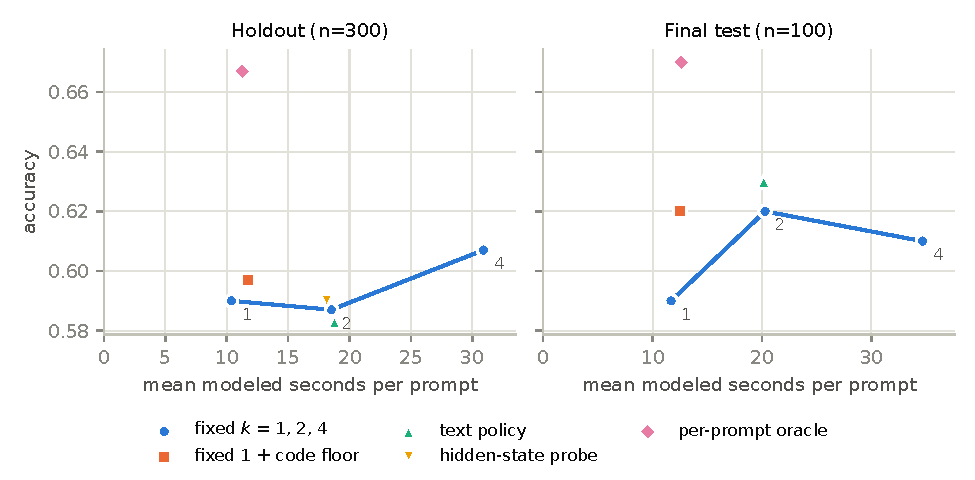
\includegraphics[width=\linewidth]{figures/fig_pareto.pdf}
\caption{Accuracy against mean modeled seconds per prompt, holdout (left) and final test (right). Fixed $k$ is flat in accuracy while cost grows with $k$. The per-prompt oracle sits well above every fixed-$k$ point at a cost close to $k{=}1$. The probe was evaluated on holdout only. The $y$-axis is shared across panels.}
\label{fig:pareto}
\end{figure}
\begin{figure}[t]
\centering
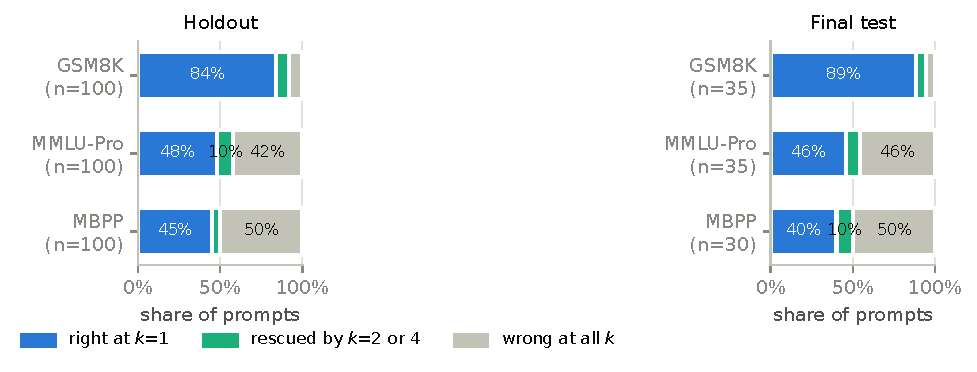
\includegraphics[width=\linewidth]{figures/fig_headroom.pdf}
\caption{Oracle decomposition by source: share of prompts already correct at $k{=}1$, correct only at $k{=}2$ or $4$ (rescued), and wrong at every $k$. Segment labels are drawn only for segments at least 13\% wide.}
\label{fig:headroom}
\end{figure}

\subsection{C2: learned routers capture none of it}
\label{sec:c2}
On holdout the text policy scores \HoldoutTextAcc\ at mean $k$ \HoldoutTextMeanK, \sg{\HoldoutTextDelta}\ versus fixed $k{=}2$ [\sg{\HoldoutTextLo}, \sg{\HoldoutTextHi}]. It fails its gate. The hidden-state probe scores \HoldoutProbeAcc\ at matched $k$, \sg{\HoldoutProbeDelta}\ [\sg{\HoldoutProbeLo}, \sg{\HoldoutProbeHi}], and is not promoted. A matched-$k$ random policy scores \HoldoutRandomAcc, which is within noise of both. On the final split the text policy scores \FinalTextAcc\ against \FinalChosenAcc\ for the chosen policy, \sg{\FinalTextDelta}\ [\sg{\FinalTextLo}, \sg{\FinalTextHi}] versus fixed $k{=}2$: noise. The conclusion is that, with these features, neither prompt text nor the $k{=}1$ last-token state predicts which prompts benefit from more loops, at the sample sizes here. We cannot rule out smaller gains or better features: the intervals are about four points wide and the training labels are noisy (Section~\ref{sec:trunc}) and heavily skewed to $k{=}1$ (the class-balance gate failed; Ruling Z).

\subsection{C3 (post hoc): fixed \texorpdfstring{$k{=}1$}{k=1} plus a code floor}
\label{sec:c3}
After the holdout results were seen we compared the heuristic ``$k{=}1$ except $k{=}2$ for code prompts''. It scores \HoldoutFloorAcc\ at \HoldoutFloorSec\ s on holdout (mean $k$ \HoldoutFloorMeanK; \sg{\HoldoutFloorDelta}\ vs fixed 2 [\sg{\HoldoutFloorLo}, \sg{\HoldoutFloorHi}]) and \FinalFloorAcc\ at \FinalFloorSec\ s on final, against \FinalFixedTwoAcc\ at \FinalFixedTwoSec\ s for fixed $k{=}2$: equal accuracy at \FloorLatencyRatio\ of the modeled latency. This is \textbf{post hoc}. The heuristic was chosen after looking at the holdout split, so the holdout number is not a clean estimate, and the final result is a single comparison on \FinalN\ prompts whose interval, \sg{\FinalFloorLo} to \sg{\FinalFloorHi}, is wide. The plan's pre-specified fallback was fixed $k{=}2$ with a code floor and that stayed the chosen policy (Ruling AB); the heuristic is reported as a comparison and a recommendation. The simplest reading of C1 and C3 together is that most of the benefit of loops is already available at $k{=}1$, and we make no stronger claim.

\begin{table}[t]
\centering\small
\begin{tabular}{lrrrr}
\toprule
Policy & Acc. & Mean $k$ & Mean s & $\Delta$ vs $k{=}2$ [95\% CI] \\
\midrule
Fixed k=1 & 0.590 & 1.00 & 10.38 & +0.003 [-0.033, +0.043] \\
Fixed k=2 & 0.587 & 2.00 & 18.52 & +0.000 [+0.000, +0.000] \\
Fixed k=4 & 0.607 & 4.00 & 30.90 & +0.020 [-0.013, +0.053] \\
Fixed k=1 + code floor & 0.597 & 1.33 & 11.76 & +0.010 [-0.027, +0.047] \\
Per-prompt oracle & 0.667 & 1.12 & 11.26 & +0.080 [+0.050, +0.113] \\
Text policy (matched $k{=}2$) & 0.583 & 2.00 & 18.77 & -0.003 [-0.020, +0.013] \\
Hidden-state probe (matched $k{=}2$) & 0.590 & 2.00 & 18.13 & +0.003 [-0.023, +0.033] \\
\bottomrule
\end{tabular}

\caption{Holdout (post-regrade), policies against fixed $k{=}2$. Modeled seconds as defined in Section~\ref{sec:setup}. The ``code floor'' rows are post hoc (C3).}
\label{tab:holdout}
\end{table}

\section{The truncation confound (C4)}
\label{sec:trunc}
A large share of MMLU-Pro outputs reach the generation cap. On holdout the truncated share is \HoldoutMmluKOneTruncRate, \HoldoutMmluKTwoTruncRate\ and \HoldoutMmluKFourTruncRate\ at $k{=}1,2,4$, against \HoldoutGsmKOneTruncRate, \HoldoutGsmKTwoTruncRate, \HoldoutGsmKFourTruncRate\ for GSM8K and \HoldoutMbppKOneTruncRate\ at every $k$ for MBPP (Figure~\ref{fig:trunc}, Table~\ref{tab:trunc}). A truncated output rarely contains an explicit final answer and is almost never graded correct, so an MMLU-Pro label of ``wrong at $k{=}1$, right at $k{=}2$'' can mean only that the answer fit under the cap at $k{=}2$. Among \emph{non-truncated} MMLU-Pro outputs, accuracy is \HoldoutMmluKOneAccNT, \HoldoutMmluKTwoAccNT\ and \HoldoutMmluKFourAccNT\ at $k{=}1,2,4$ (all-item accuracy is in Table~\ref{tab:persource}), but these are \emph{conditional} on fitting, and the set of items that fit changes with $k$, so the three figures are not a like-for-like comparison and we do not interpret their trend as a loop effect.

This limits both C1 and C2. MMLU-Pro is one third of the labelled data, a large share of its labels measure answer length, and a router trained on them is partly learning to predict length. The oracle's gain on MMLU-Pro (Table~\ref{tab:persource}) may therefore be inflated by truncation. We did not re-sweep MMLU-Pro with a larger cap (Ruling AF): it would take several GPU-hours and the final split's one-shot evaluation was already spent. Whether the null result in C2 survives a cap that does not truncate is an open question and the most useful next experiment.

\begin{figure}[t]
\centering
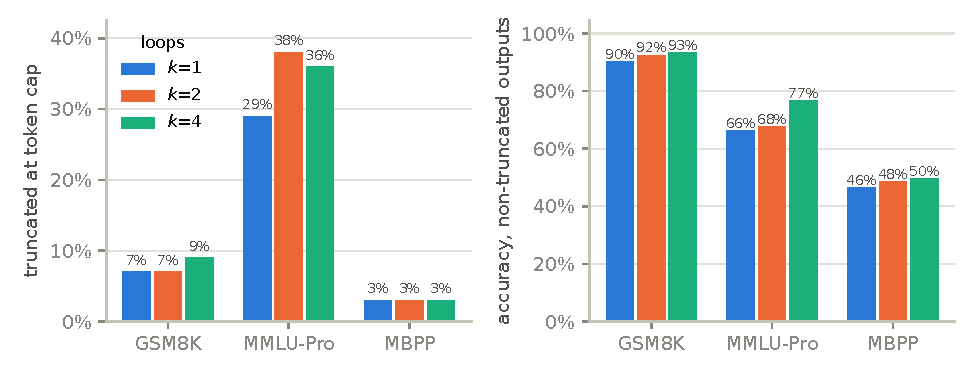
\includegraphics[width=\linewidth]{figures/fig_truncation.pdf}
\caption{Holdout only. Left: share of outputs truncated at the generation cap. Right: accuracy among non-truncated outputs. Training cells are omitted because lazy labelling makes their $k{=}2,4$ items a failure-selected subset.}
\label{fig:trunc}
\end{figure}

\section{Systems on Apple silicon (C5)}
\label{sec:systems}
\paragraph{Self-speculative decoding from a same-weights draft.}
llama.cpp supports a separate draft model. Because the draft needs only a different loop count, we made it by cloning the stock GGUF (an APFS copy-on-write clone, so no extra disk) and setting \texttt{dory.num\_loops=1}; the target is the stock GGUF with metadata $k{=}4$ (Ruling AH). The server must be started with \texttt{--spec-type draft-simple}; the default does nothing (Ruling AI). In an interleaved A/B (Section~\ref{sec:measure}) over \SpecPrompts\ holdout prompts, a draft length of four tokens gives a geometric-mean speedup of \SpecNFourSpeedup$\times$ over plain $k{=}4$ decoding (95\% CI \SpecNFourLo--\SpecNFourHi; faster on \SpecNFourFaster\ of \SpecPrompts\ prompts), with draft acceptance \SpecNFourAccept\ and outputs identical to plain decoding on \SpecNFourIdentical\ of \SpecPrompts. A draft length of six gives \SpecNSixSpeedup$\times$ (\SpecNSixLo--\SpecNSixHi) but lower acceptance, \SpecNSixAccept. The intervals overlap; we kept four because six did not meet the pre-set acceptance bar (Ruling AN). A per-prompt best-draft-length oracle bounded the possible gain of a confidence-driven draft length at a few percent, so we did not patch llama.cpp for it (Ruling AM). Draft models with more loops, and a CPU draft, were slower. Speedups are only relevant when a request is routed to $k{=}4$; the chosen policy never starts a $k{=}4$ server, so this result is independent of the controller.

\paragraph{Negative results.}
N-gram lookup drafting (\texttt{ngram-simple}) on MBPP prompts that included the reference solution as context ran at \NgramSpeedup$\times$ plain speed. Running \LayersGpu\ of \LayersAll\ layers on the GPU and the rest on the CPU ran at \OffloadSpeedup$\times$ with the same graded accuracy; full GPU offload stays. A q8\_0 KV cache at $k{=}4$ on \QEightN\ holdout GSM8K and MMLU-Pro prompts scored \QEightAcc\ against \QSixteenAcc\ for f16 (change \sg{\QEightDelta}), failing the one-point gate, so f16 stays (it would save about one and a half GB per server if memory were short).

\paragraph{Controller overhead and the Neural Engine.}
Running the NVIDIA classifier in PyTorch on the GPU takes about \MpsMs\,ms per request (\CpuMs\,ms on CPU). Converting it to Core~ML for the Neural Engine takes \AneMs\,ms, \AneSpeedup$\times$ faster, with identical argmax on every head over \AneN\ holdout prompts (fp16; other Core~ML compute units returned NaN logits and are unusable as converted). In the live router the chosen policy added \LiveOverheadMs\,ms per request on \LiveGateN\ holdout prompts, with zero accuracy disagreement against the offline run, and the router serializes classifier calls with a lock. The Core~ML path was not wired into the router: it saves a negligible fraction of a request's latency and costs more memory and a crash-prone dependency (Ruling AO).

\begin{figure}[t]
\centering
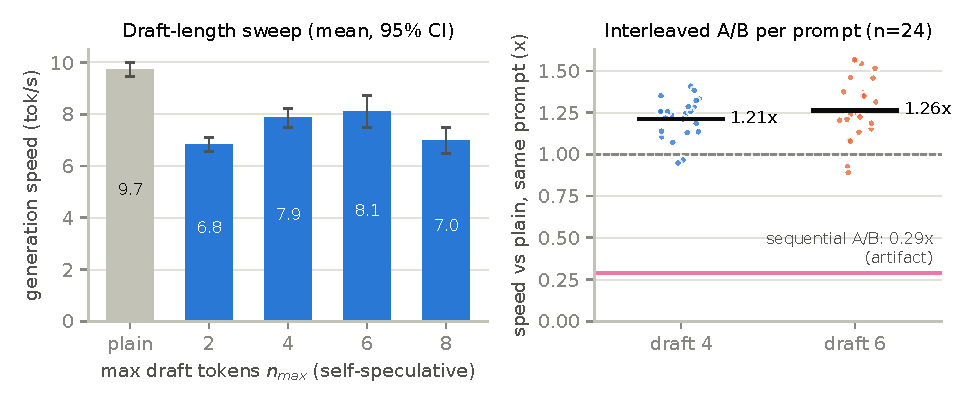
\includegraphics[width=\linewidth]{figures/fig_spec.pdf}
\caption{Self-speculative decoding. Left: draft acceptance from the draft-length sweep. The sweep ran its configurations sequentially, so its throughput is load-confounded and only acceptance is shown. $n_{\max}=8$ with ``(p07)'' is \texttt{--spec-draft-n-max 8 --spec-draft-p-min 0.7}; its acceptance is not comparable with the others because the probability threshold makes it draft fewer tokens. Right: per-prompt speed relative to plain decoding from the interleaved A/B; bars are geometric means. The horizontal line at \SpecSequentialRatio$\times$ is the sequential-arm artifact discussed in Section~\ref{sec:measure}.}
\label{fig:spec}
\end{figure}

\section{Measuring on a shared laptop (C6)}
\label{sec:measure}
Our first speculative benchmark ran the speculative and plain arms one after the other. It gave acceptance \SpecSequentialAccept\ and identical outputs but a speed of \SpecSequentialRatio$\times$ plain: apparently a large slowdown. The arms had run hours apart; a controlled re-run did not reproduce it (Ruling AK). The draft-length sweep, also sequential, then showed that a clean sequential plain re-run was faster than every speculative arm, which could not be true, and plain rows written while we ran diagnostics were contaminated and discarded (Ruling AL). We attribute the drift to uncontrolled background load on a shared laptop; we did not isolate its source.

The fix is to interleave: all servers are up, and for each prompt the arms run back to back with their order rotated, so slow periods hit every arm. Speed is then a per-prompt ratio, summarized by its geometric mean with a bootstrap interval. That gave \SpecNFourSpeedup$\times$ for the $n{=}4$ draft. A four-server variant crashed Metal with a compute error, so the final A/B ran with three servers up. The lesson is general: on a shared machine, sequential A/B measures the machine's drift as much as the treatment, and the ratio can land far outside the plausible range with identical outputs and sensible acceptance.

\section{Limitations}
\begin{itemize}
\item One machine (Apple M4, \MemGb\,GB), one model (Dory1.0-4B), one quantization (Q5\_K\_M), one backend (Metal) that the PR's authors list as untested, and a pinned build of an unmerged PR.
\item Greedy decoding with thinking disabled. The card recommends temperature 1.0, top-p 0.95 and reasoning on, and its benchmarks use BF16 weights; our accuracy levels are not comparable to the card's and the null result might not transfer to sampled or reasoning-mode decoding.
\item Small evaluation sets (\HoldoutN\ holdout, \FinalN\ final) with intervals of about four to eight points; effects of one or two points are below resolution.
\item MMLU-Pro labels are truncation-bound (C4); we did not re-sweep with a larger cap.
\item The grader was changed after the main runs and the final split was evaluated twice. The change was applied identically to all splits and both versions are reported, but a reader should note that it happened.
\item C3 was found after seeing the holdout split. The oracle is optimistic because it selects among noisy runs.
\item Modeled seconds rank policies by requested compute and ignore queueing, batching and load. The speculative speedup is measured on \SpecPrompts\ prompts with \SpecTokens\ generated tokens. Only $k{=}4$ is sped up; the chosen policy does not use it.
\item Only features available before generation were tried. We did not try per-token control, fine-tuning for routing, or mid-layer probes.
\end{itemize}

\section{Related work}
Looped and recurrent-depth models include Huginn \citep{huginn2025}, Ouro \citep{ouro2025} and Dory \citep{dory2026}; Ouro trains a learned depth-allocation objective, whereas we study per-request control of a model whose loop count is a serving-time setting. CDB addresses batching of depth-adaptive looped models \citep{cdb2026}. Self-speculative decoding drafts from the same model by skipping layers or exiting early \citep{draftverify2024,layerskip2024}, building on speculative decoding \citep{leviathan2023}; our draft uses the same weights with fewer loops, via GGUF metadata. The router's text features come from a public prompt-task classifier \citep{nvclassifier}. Laya is a related typed-decision model with a self-reported forward time of about $33$\,ms on a T4 and is not generative \citep{laya}; we mention it only as a latency reference point for small decision models. Support for Dory in vLLM has been merged \citep{vllm60149}; we did not test it.

\section{Conclusion}
For Dory1.0-4B on a laptop, with greedy decoding and a truncation-aware grader, fixed loop count barely changes accuracy and costs roughly in proportion to $k$. Per-prompt headroom exists on paper, but neither prompt-text features nor a hidden-state probe capture it, and a cheap two-rule heuristic found after the fact does as well as fixed $k{=}2$ at about \FloorLatencyRatio\ of the latency, which we report as post hoc. A truncation confound limits what the MMLU-Pro labels can say. On the systems side, a same-weights $k{=}1$ draft gives \SpecNFourSpeedup$\times$ with identical outputs, other offload tricks lose, and interleaved measurement is necessary on a shared laptop. Code, results and the generation scripts for every number and figure are in the repository.

\bibliographystyle{plainnat}
\bibliography{refs}

\appendix
\section{Protocol rulings}
\label{app:rulings}
Every recorded decision made while running the study, with its rationale. Letters are the identifiers in \texttt{results/decisions.md}.
\begin{description}\small\setlength{\itemsep}{2pt}
\item[A] The first task was split so a shared scaffold (package skeleton, configuration, test fixtures) landed before parallel work began, avoiding conflicting edits.
\item[B] The loop counts $\{1,2,4\}$ and the code floor of two live in one configuration module so labels and policies cannot disagree.
\item[C] The Python environment reuses the globally installed torch, transformers, scikit-learn and datasets, to avoid duplicate multi-gigabyte installs.
\item[D] Runs longer than about fifteen minutes are launched detached and kept awake, with logs under \texttt{results/logs}, so they survive session limits and sleep.
\item[E] Work proceeded with about twelve GB of free disk, with downloads required to abort if free space fell below eight GB.
\item[F] The integration test against a real server stays skipped until the weights and build exist, then runs after merge.
\item[G] Implementer and reviewer instructions are stored as files and reused verbatim so every task is built and reviewed under the same contract.
\item[H] Parallel work branches merge only after the build and weight-fetch task finishes, so tests run against a complete tree.
\item[I] Two minor review findings were promoted to required fixes before merging.
\item[J] The grader is hardened against formatting: code-fence variants, a prose-letter fallback and missing-boundary handling for MMLU-Pro, and for GSM8K an explicit ``answer is $N$'' preferred over the last number.
\item[K] Controller work was split into code first and training plus gate later, after labels exist; classifier weights are not downloaded until needed because of disk.
\item[L] Markdown-formatted MMLU-Pro answers (for example bold ``Answer: C'') are graded as answers.
\item[M] The answer-prefix pattern was tightened so ordinary prose is not read as an answer.
\item[N] The baseline quality run and the hidden-state feature extraction were split from their code, to run when their dependencies finish.
\item[O] A classifier-loading error exposed only by the real model was fixed immediately instead of waiting for the task that depended on it.
\item[P] Transient server errors are retried; an error row counts as finished only if it carries a grade or an HTTP 4xx, and downstream code uses the last clean row per item, loop count and variant.
\item[Q] The memory gate is measured as system-wide memory and swap change, with swap growth at most one GB, instead of summed process memory, because memory-mapped weights are shared between servers.
\item[R] Raw prompt text, without a ``Prompt:'' prefix, is fed to the classifier.
\item[S] The label-sweep and live-router tasks were split into code and run phases. Speculative decoding was skipped at that point because llama-server copied the target's metadata overrides into the draft; this was reversed later (AH).
\item[T] The default generation cap is \CapText\ tokens with \CapCode\ for MBPP, which needs longer outputs; a mismatch risk in the loop-count parameter was fixed with routing tests.
\item[U] Each sweep is re-run, up to two extra passes, until no transient-error rows remain before labels are built.
\item[V] The f16 KV cache was chosen and the q8\_0 quality check initially skipped because memory was not tight. The check was run later (Section~\ref{sec:systems}); f16 stays.
\item[W] The long sweeps were chained in a script and launched in the background after the code was merged.
\item[X] The baseline quality gate was analyzed directly rather than delegated.
\item[Y] A tie counts as passing a gate that is stated as at least.
\item[Z] Work continued past the failed class-balance gate (every class share at most \GateClass; the $k{=}1$ share was larger). The classifier is class-weighted, and the later gate against fixed $k{=}2$ is the real test of usefulness; a negative result there is the answer.
\item[AA] A label-dtype bug (object arrays from missing labels) was fixed, with a regression test.
\item[AB] The plan's fallback, fixed $k{=}2$ with a code floor, is kept as the chosen policy even though fixed $k{=}1$ with a code floor scored better on holdout; the latter is reported on final as a comparison only. This is why C3 is post hoc.
\item[AC] The live-router gate and the final test were run with two small scripts rather than delegated.
\item[AD] The router holds a lock around the classifier because the GPU classifier is not thread-safe.
\item[AE] The controller-overhead failure is accepted: the text policy exceeded its overhead budget and the chosen policy's \LiveOverheadMs\,ms is a tiny fraction of a request, and the text policy is not deployed.
\item[AF] The review follow-up was limited to documentation (truncation caveat and per-source breakdown). MMLU-Pro was not re-swept with a larger cap because it needs several GPU-hours and the final split's one-shot evaluation was already spent.
\item[AG] Remaining code minor issues were initially left: the chosen policy still runs the classifier for the code flag, the memory gate did not cover a learned-policy router, and last-number grader false positives of about half a point. The grader item was later addressed by the truncation-aware regrade, which skips MBPP.
\item[AH] The draft model is an APFS clone of the stock GGUF with \texttt{dory.num\_loops=1}; the target is the stock GGUF with no override, because llama-server copies target overrides into the draft. If wrong, speedups would be mismeasured; an output-identity check guards this.
\item[AI] \texttt{--spec-type draft-simple} is required; the default loads the draft but never drafts.
\item[AJ] Re-running the final test after a grader correction is allowed: the one-shot rule guards against tuning on the final split, and a fix applied identically to all splits is not tuning. Both versions are recorded; the headline moves by about two items.
\item[AK] The \SpecSequentialRatio$\times$ result is a measurement artifact: the arms ran hours apart, likely under external GPU load. The verdict on speed was deferred to back-to-back measurement.
\item[AL] Plain-decoding rows written while diagnostics were running in the draft sweep were deleted and re-run.
\item[AM] The draft length stays at four; a confidence-driven length is not worth a llama.cpp patch given a ceiling of a few percent within run noise.
\item[AN] The speculative gate (acceptance at least \GateAcc, speedup at least \GateSpeed$\times$, identical outputs) passes with $n{=}4$. Six drafts fail the acceptance bar and the intervals overlap, so four is kept.
\item[AO] The Core~ML classifier is not wired into the router: it saves a few tens of milliseconds per request, a tiny fraction of a typical request, at the cost of more memory and a crash-prone dependency.
\end{description}

\section{Full tables}
\begin{table}[h]
\centering\small
\begin{tabular}{lrrrr}
\toprule
Policy & Acc. & Mean $k$ & Mean s & $\Delta$ vs $k{=}2$ [95\% CI] \\
\midrule
Fixed k=1 & 0.590 & 1.00 & 11.69 & -0.030 [-0.090, +0.030] \\
Fixed k=2 & 0.620 & 2.00 & 20.28 & +0.000 [+0.000, +0.000] \\
Fixed k=4 & 0.610 & 4.00 & 34.67 & -0.010 [-0.060, +0.040] \\
Fixed k=1 + code floor & 0.620 & 1.30 & 12.51 & +0.000 [-0.050, +0.050] \\
Per-prompt oracle & 0.670 & 1.12 & 12.61 & +0.050 [+0.010, +0.100] \\
Text policy & 0.630 & 1.92 & 20.16 & +0.010 [-0.020, +0.040] \\
\bottomrule
\end{tabular}

\caption{Final split ($n{=}\FinalN$, post-regrade). The code-floor row is post hoc (C3); the text row is a reference and not a deployed policy.}
\end{table}
\begin{table}[h]
\centering\scriptsize
\resizebox{\linewidth}{!}{\begin{tabular}{lrrrrrrrrrr}
\toprule
Source & \multicolumn{2}{c}{Fixed k=1} & \multicolumn{2}{c}{Fixed k=2} & \multicolumn{2}{c}{Fixed k=4} & \multicolumn{2}{c}{Fixed k=1 + code floor} & \multicolumn{2}{c}{Per-prompt oracle} \\
 & Acc. & s & Acc. & s & Acc. & s & Acc. & s & Acc. & s \\
\midrule
GSM8K ($n{=}100$) & 0.840 & 12.0 & 0.860 & 20.6 & 0.850 & 34.3 & 0.840 & 12.0 & 0.920 & 12.7 \\
MMLU-Pro ($n{=}100$) & 0.480 & 14.4 & 0.430 & 26.0 & 0.490 & 44.4 & 0.480 & 14.4 & 0.580 & 15.9 \\
MBPP ($n{=}100$) & 0.450 & 4.8 & 0.470 & 8.9 & 0.480 & 14.1 & 0.470 & 8.9 & 0.500 & 5.1 \\
\bottomrule
\end{tabular}
}
\caption{Holdout accuracy and mean modeled seconds by source.}
\label{tab:persource}
\end{table}
\begin{table}[h]
\centering\small
\begin{tabular}{llrrrr}
\toprule
Split & Source, $k$ & $n$ & Truncated & Acc. (non-trunc.) & Acc. (all) \\
\midrule
holdout & GSM8K, 1 & 100 & 0.070 & 0.903 & 0.840 \\
holdout & GSM8K, 2 & 100 & 0.070 & 0.925 & 0.860 \\
holdout & GSM8K, 4 & 100 & 0.090 & 0.934 & 0.850 \\
holdout & MMLU-Pro, 1 & 100 & 0.290 & 0.662 & 0.480 \\
holdout & MMLU-Pro, 2 & 100 & 0.380 & 0.677 & 0.430 \\
holdout & MMLU-Pro, 4 & 100 & 0.360 & 0.766 & 0.490 \\
holdout & MBPP, 1 & 100 & 0.030 & 0.464 & 0.450 \\
holdout & MBPP, 2 & 100 & 0.030 & 0.485 & 0.470 \\
holdout & MBPP, 4 & 100 & 0.030 & 0.495 & 0.480 \\
train & GSM8K, 1 & 600 & 0.078 & 0.915 & 0.845 \\
train & GSM8K, 2 & 93 & 0.333 & 0.645 & 0.430 \\
train & GSM8K, 4 & 53 & 0.396 & 0.406 & 0.245 \\
train & MMLU-Pro, 1 & 600 & 0.410 & 0.638 & 0.387 \\
train & MMLU-Pro, 2 & 368 & 0.641 & 0.303 & 0.117 \\
train & MMLU-Pro, 4 & 325 & 0.702 & 0.155 & 0.049 \\
train & MBPP, 1 & 300 & 0.023 & 0.614 & 0.600 \\
train & MBPP, 2 & 120 & 0.058 & 0.133 & 0.125 \\
train & MBPP, 4 & 105 & 0.029 & 0.039 & 0.038 \\
\bottomrule
\end{tabular}

\caption{Truncation by split, source and $k$. Training rows at $k{=}2,4$ cover only items that failed at $k{=}1$ (lazy labelling) and are not comparable across $k$.}
\label{tab:trunc}
\end{table}
\begin{table}[h]
\centering\small
\begin{tabular}{lrl}
\toprule
Configuration & Speed vs plain & Notes \\
\midrule
Self-speculative, draft 4 & 1.21$\times$ [1.16, 1.26] & acceptance 0.84, outputs identical \\
Self-speculative, draft 6 & 1.26$\times$ [1.19, 1.34] & acceptance 0.76, outputs identical \\
n-gram lookup (MBPP) & 0.74$\times$ & \\
Partial GPU offload (54/72 layers) & 0.93$\times$ & same graded accuracy \\
Sequential A/B (artifact) & 0.29$\times$ & arms hours apart under varying load \\
Core ML (Neural Engine) classifier & 2.5$\times$ & 17.9 vs 44.3 ms (MPS) \\
\bottomrule
\end{tabular}

\caption{Systems results. Speed ratios for speculative decoding are per-prompt geometric means from the interleaved A/B; the sequential row is an artifact.}
\end{table}
\end{document}
